\chapter{\chatextbasisCalculus}\label{cha:basisCalculus}

Basis Calculus stores informations in the selection of basis elements, while coordinate calculus uses the coordinates to each index for storage.
While coordinate calculus is more expressive, basis calculus can be exploited in sparse representations of composed functions.

%\sect{Classification of tensors}

We frequently worked in \parref{par:one} and \parref{par:two} with tensors, which have non-negative coordinates and occasionally are boolean (see \defref{def:booleanTensor}) or directed (see \defref{def:directedTensor}).
While boolean tensors have appeared as semantical representation of formulas, directed tensors have appeared mostly as conditional distributions.
In this chapter we provide further insights into the situation, where tensors satisfy both.
For a schematic depiction of this see \figref{fig:dbTensorSketch}.

\begin{figure}[h]
	\begin{center}
		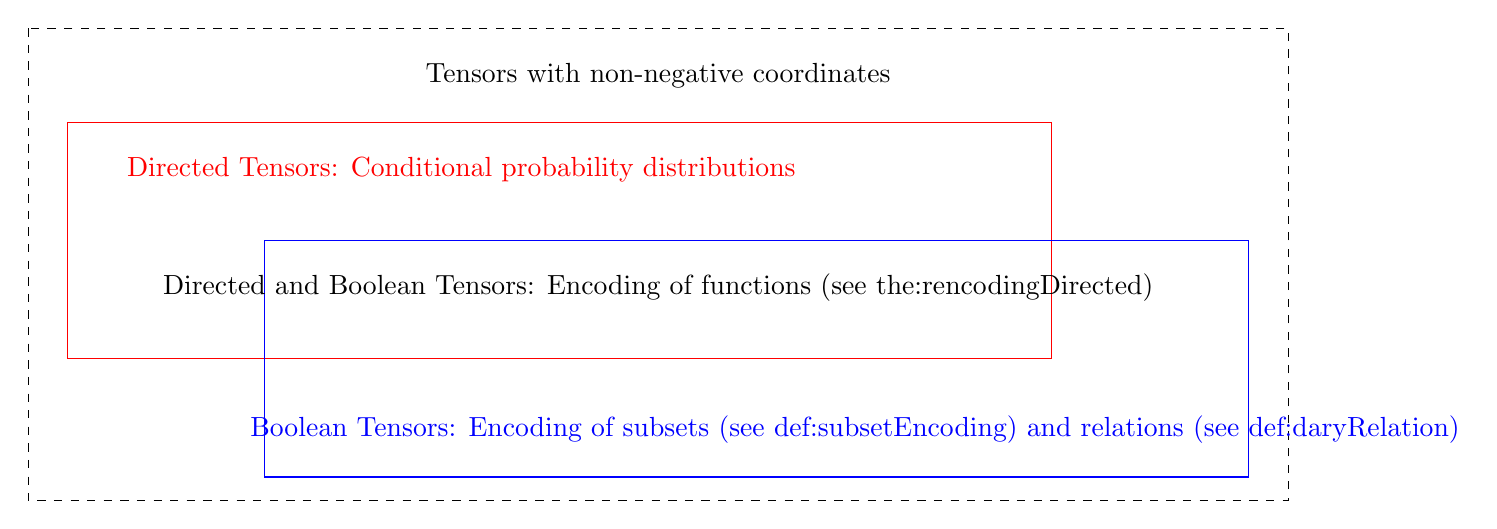
\begin{tikzpicture}[yscale=0.6]
	\draw[dashed] (-10.5,12) rectangle (5.5,2);
	\node[anchor=center] (text) at (-2.5,11) {Tensors with non-negative coordinates};
	
	\draw[red] (-10,10) rectangle (2.5,5); 
	\node[anchor=center,red] (text) at (-5,9) {Directed Tensors: Conditional probability distributions};
	\draw[blue] (-7.5,7.5) rectangle (5,2.5); 
	\node[anchor=center,blue] (text) at (0,3.5) {Boolean Tensors: Encoding of subsets (see \defref{def:subsetEncoding}) and relations (see \defref{def:daryRelation})};

	\node[anchor=center] (text) at (-2.5,6.5) {Directed and Boolean Tensors: Encoding of functions (see \theref{the:rencodingDirected})};
\end{tikzpicture}
	\end{center}
	\caption{Sketch of the tensors with non-negative coordinates.
	We investigate in this chapter tensors, which are directed and boolean.}\label{fig:dbTensorSketch}
\end{figure}



\sect{Encoding of Subsets and Relations}

Based on the concept of one-hot encodings of states we in this chapter develop the construction of encodings to sets, relations and functions.
We start with the definition of subset encodings, which represent set memberships in their boolean coordinates.

\begin{definition}[Subset Encoding]\label{def:subsetEncoding}
	We say that an arbitrary set $\arbset$ is enumerated by an enumeration variable $\indvariableof{\arbset}$ taking values in $[\inddimof{\arbset}]$, when $\inddimof{\arbset}=\absof{\arbset}$ and there is a bijective index interpretation function
	\begin{align*}
		\indexinterpretation : [\inddimof{\arbset}] \rightarrow \arbset \, .
	\end{align*}
	Given an set $\arbset$ enumerated by the variable $\indvariableof{\arbset}$, any subset $\arbsubset\subset\arbset$ is encoded by the tensor $\onehotmapto{\arbsubset}[\indvariable]$ defined for $\indindex\in[\absof{\arbset}]$ as
	\begin{align*}
	 	\onehotmapofat{\arbsubset}{\indexedindvariable}
		= \begin{cases}
		1 & \text{if} \indexinterpretationat{\indindex} \in \arbsubset \\
		0 & \text{else}
		\end{cases} \, .
	\end{align*}
\end{definition}

% Decomposition
In a one-hot basis decomposition we have
\begin{align*}
	\onehotmapofat{\arbsubset}{\indvariable}
	\coloneqq \sum_{\indindex\in[\cardof{\arbset}]\,:\,\indexinterpretationat{\indindex}\in\arbsubset}\onehotmapofat{\indindex}{\indvariable} \, .
\end{align*}

% Explanation
%Encoding of subsets as vectors: Each coordinate associated with a possible element, $\{0,1\}$ encoding whether in subset.
%The encodings is thus a boolean tensor.
%Any subset encoding is a boolean tensor.

% Relation
Since relations are subsets of cartesian products between two sets, their encoding is a straightforward generalization of \defref{def:subsetEncoding}.

\begin{definition}[Relation Encoding]
	A relation between two finite sets $\inset$ and $\outset$ is a subset of their cartesian product
	\begin{align*}
		 \exrelation \subset \inset \times \outset \, .
	\end{align*}
	Given an enumeration of $\inset$ and $\outset$ by the categorical variables $\indvariableof{\insymbol}$ and $\indvariableof{\outsymbol}$ and interpretation maps $\indexinterpretationof{\insymbol}$, $\indexinterpretationof{\outsymbol}$, we define the encoding of this subset as the tensor $\onehotmapto{\exrelation}[\indvariableof{\insymbol},\indvariableof{\outsymbol}]$ with the coordinates
	\begin{align*}
		\onehotmapofat{\exrelation}{\indexedindvariableof{\insymbol},\indexedindvariableof{\outsymbol}}
		= \begin{cases}
		1 & \text{if } (\indexinterpretationofat{\insymbol}{\indindexof{\insymbol}},\indexinterpretationofat{\outsymbol}{\indindexof{\outsymbol}}) \in \exrelation \\
		0 & \text{else}
		\end{cases} \, .
	\end{align*}
\end{definition}

% Decomposition
The relation encoding has a decomposition into one-hot encodings as
\begin{align*}
	\onehotmapofat{\exrelation}{\indvariableof{\insymbol},\indvariableof{\outsymbol}}
	= \sum_{\indindexof{\insymbol},\indindexof{\outsymbol} \, : \, (\indexinterpretationofat{\insymbol}{\indindexof{\insymbol}},\indexinterpretationofat{\outsymbol}{\indindexof{\outsymbol}}) \in \exrelation}
	\onehotmapofat{\indindexof{\insymbol}}{\indvariableof{\insymbol}}  \otimes \onehotmapofat{\indindexof{\outsymbol}}{\indvariableof{\outsymbol}}  \, .
\end{align*}

Relational encodings have a matrix structure by the cartesian product, which can be further folded to tensors, when the sets itself are cartesian products.
The relational encoding is a bijection between the relations of two sets and the boolean tensors with their enumeration variables.

%They provide representations of generic relations by boolean tensors, in the sense that each relation between two sets is represented
%\begin{theorem}
%	The relational encoding is a bijection between the set of relations and the set of boolean tensors.
%\end{theorem}
%\begin{proof}
%	% =>
%	By definition, a relational encoding is the encoding of a subset and thus a boolean tensor.
%	% <=
%	Any matrification of a boolean tensor marks by its $1$ coordinates the elements of a relation.
%\end{proof}
%
%% Significance
%We can thus understand any matrification of a boolean tensor as the encoding of a relation and vice versa.



\subsect{Higher order relations}

We can extend this contraction to relations of higher order, and arrive at encoding schemes usable for relational databases.

\begin{definition}\label{def:daryRelation}
	Given sets $\arbsetof{\atomenumerator}$ for $\atomenumeratorin$, a $\atomorder$-ary relation is a subset of a their cartesian product, that is
	\begin{align*}
		\exrelation \subset\bigtimes_{\atomenumeratorin} \arbsetof{\atomenumerator} \, .
	\end{align*}
	Given an enumeration of each set $\arbsetof{\atomenumerator}$ by a variable $\indvariableof{\atomenumerator}$ and an interpretation map $\indexinterpretationof{\atomenumerator}$, we define the encoding of the relation as the tensor $\onehotmapto{\exrelation}[\indvariableof{[\atomorder]}]$ with coordinates
	\begin{align*}
		\onehotmapofat{\exrelation}{\indexedindvariableof{[\catorder]}}
		= \begin{cases}
		1 & \text{if} \quad (\indexinterpretationofat{0}{\indindexof{0}},\ldots,\indexinterpretationofat{\atomorder-1}{\indindexof{\atomorder-1}}) \in \exrelation \\
		0 & \text{else}
		\end{cases} \, .
	\end{align*}
\end{definition}

\begin{example}[Propositional Formulas]
	Let there be for $\atomenumeratorin$ sets $\arbsetof{\atomenumerator}$ of truth assignments to the $\atomenumerator$-th atom, which are all enumerated by $[2]$.
	A propositional formula then corresponds with a $\atomorder$-ary relation and we directly defined them in \defref{def:formulas} by their relational encoding.
\end{example}

\begin{example}[Relational Databases]
	Relational Databases can be encoded as tensors using the relation encoding scheme.
	Each column is thereby understood as an eunumeration variable, which values form the sets $\arbsetof{\catenumerator}$.
\end{example}

% Sparse Representations
Let us notice, that the dimensionality of the tensor space used for representing a relation is
\begin{align*}
	\prod_{\catenumeratorin} \cardof{\arbsetof{\catenumerator}}
\end{align*}
and therefore growing exponentially with the number of variables.
Relations are however often sparse, in the sense that
\begin{align*}
	 \cardof{\exrelation} << \prod_{\catenumeratorin} \cardof{\arbsetof{\catenumerator}} \, .
\end{align*}
It is therefore often benefitially to choose sparse encoding schemes, for example by restricted CP formats (see \charef{cha:sparseCalculus}) to represent $\onehotmapof{\exrelation}$.


\sect{Encoding of Functions}

Let us now restrict to relations, which have an expression by functions.
We in this section then show, how contractions of their encodings can be exploited in function evaluation.

\subsect{Relational Encoding of Functions}

%We now generalize the representation scheme towards maps between arbitrary unstructured sets.

\begin{definition}[Relational Encoding of Maps]\label{def:functionRelationEncoding}
	Any map
	\begin{align*}
		\exfunction : \inset \rightarrow \outset
	\end{align*}
	can be represented by a relation
	\begin{align*}
		\exrelationof{\exfunction} \coloneqq \left\{ (x,\exfunction(x) \, : \, x \in\inset )\right\} \subset \inset \times \outset \, .
	\end{align*}
	Given a enumeration of the sets by $\indvariableof{\insymbol}$ and $\indvariableof{\outsymbol}$ we define the relational encoding of $\exfunction$ as the tensor
	\begin{align*}
		\rencodingofat{\exfunction}{\indvariableof{\insymbol},\indvariableof{\outsymbol}}
		= \onehotmapofat{\exrelationof{\exfunction}}{\indvariableof{\insymbol},\indvariableof{\outsymbol}}  \, .
	\end{align*}
\end{definition}

\begin{remark}[Reduction to images]
	% Image enumeration
	When $\exfunction$ maps into a set of infinite cardinality, we restrict $\outset$ to the image of $\exfunction$ and enumerate the image by a variable $\indvariableof{\exfunction}$.
	This scheme is applied, when $\exfunction$ is itself a tensor, i.e. $\outset=\rr$.
	While the variable $\indvariableof{\exfunction}$ can in general be of the same cardinality as the domain set $\inset$, it will be valued in $[2]$ when considering boolean tensors.
\end{remark}

% Characterization of the directed and boolean tensors
We notice, that any relational representation of a function is also a directed tensor with incoming variables to the domain and outgoing variables to the image.
It furthermore holds, that the set of directed and boolean tensors is characterized by the relational encoding of functions.
This is shown in the next theorem, by the claim that any boolean tensor which is directed is the relational representation of a function.

\begin{theorem}\label{the:rencodingDirected}
	Let $\inset,\outset$ be sets and $\exrelation\subset\inset\times\outset$ a relation.
	If and only if there exists a map $\exfunction:\inset\rightarrow\outset$ such that $\exrelation=\exrelationof{\exfunction}$, the relational encoding $\rencodingof{\exfunction}$ is a directed tensor with $\indvariableof{\insymbol}$ incoming and $\indvariableof{\outsymbol}$ outgoing.
\end{theorem}
\begin{proof}
	\proofrightsymbol:
	When $\exfunction$ is a function, we have for any $\indindexofin{\insymbol}$
	\begin{align*}
		\sum_{\indindexofin{\outsymbol}} \rencodingofat{\exfunction}{\indexedindvariableof{\insymbol},\indexedindvariableof{\outsymbol}}
		=  \rencodingofat{\exfunction}{\indexedindvariableof{\insymbol},\indvariableof{\outsymbol}=\invindexinterpretationofat{\outsymbol}{\exfunctionat{\indexinterpretationofat{\insymbol}{\indindexof{\insymbol}}}}}
		= 1 \, .
	\end{align*}
	Thus, $\rencodingofat{\exfunction}{\indvariableof{\outsymbol},\indvariableof{\insymbol}}$ is a directed tensor with variables $\indvariableof{\insymbol}$ incoming and $\indvariableof{\outsymbol}$ outgoing.

	\proofleftsymbol:
	Conversely let there be a relation $\exrelation$, such that $\rencodingof{\exrelation}$ is directed.
	To this end, we observe that for any $\indindexofin{\insymbol}$ the tensor
	\begin{align*}
		\onehotmapofat{\exrelation}{\indexedindvariableof{\insymbol},\indvariableof{\outsymbol}}
	\end{align*}
	is a boolean tensor with coordinate sum one and therefore a basis vector.
	It follows that the function $\exfunction : \inset \rightarrow \outset $ defined for $x\in\inset$ as
	\begin{align*}
		\exfunctionat{x}
		= \indexinterpretationofat{\outsymbol}{\invonehotmapof{\onehotmapofat{\exrelation}{\indvariableof{\insymbol}=\indexinterpretationofat{\insymbol}{x},\indvariableof{\outsymbol}}}}
	\end{align*}
	is well-defined.
	We then have by construction
	\begin{align*}
		\rencodingofat{\exfunction}{\indvariableof{\outsymbol},\indvariableof{\insymbol}}
		& = \sum_{\indindexofin{\insymbol}}
		\onehotmapofat{\exfunction(\indindexof{\insymbol})}{\indvariableof{\outsymbol}} \otimes
		\onehotmapofat{\indindexof{\insymbol}}{\indvariableof{\insymbol}} \\
		& =  \sum_{\indindexofin{\insymbol}} \onehotmapofat{\exrelation}{\indexedindvariableof{\insymbol},\indvariableof{\outsymbol}} \otimes
		\onehotmapofat{\indindexof{\insymbol}}{\indvariableof{\insymbol}} \\
		& = \onehotmapofat{\exrelation}{\indvariableof{\outsymbol},\indvariableof{\insymbol}}
	\end{align*}
	and therefore by \defref{def:functionRelationEncoding} $\exrelation=\exrelationof{\exfunction}$.
\end{proof}

% Grid sets
We are specially interested in sets of states of a factored system, which amounts to the case in \defref{def:functionRepresentation}.
Those state sets have a decomposition into a cartesian product of $\atomorder$ sets
	\[ \arbset = \facstates \, . \]
The most obvious enumeration of the set $\arbset$ is therefore by the collection of state variables $\{\catvariableof{\atomenumerator} \, : \, \atomenumeratorin \}$.
Functions between states of factored systems with $\atomorder_{\insymbol}$ and $\atomorder_{\outsymbol}$ state variables can be represented by $\atomorder_{\insymbol}+\atomorder_{\outsymbol}$-ary relations and \defref{def:functionRelationEncoding} has an obvious generalization to this case with multiple enumeration variables.

%% NOT NEEDED -> Done in propositional logics
%% Conditional
%Since the relational encoding of any map between factored systems is directed, it can be interpreted by a conditional probability tensor, as we state next.
%
%%% Maps
%\begin{corollary}%\label{the:condProbFunctionRepresentation}
%	The relational encoding $\rencodingof{\exfunction}$ (see \defref{def:functionRepresentation}) of a function $\exfunction$ between factored systems is a conditional probability tensor, where the legs to the image system are the conditions and the legs to the target system the distribution legs.
%\end{corollary}
%
%%% Deterministic by construction
%These are deterministic conditional probability tensors, in the sense that any slice with respect to the input variables is a basis tensor.
%Through contractions with distribution tensors (e.g. distributions in domain systems) they get stochastic.
%This is for example the case in the empirical distribution, which can be understood as the forwarding of the uniform distribution on the sample enumeration.

\subsect{Function Evaluation}

We now justify the nomenclature of basis calculus, by showing that contraction with basis elements produce the one-hot encoded function evaluation.

\begin{theorem}[Function evaluation in Basis Calculus]\label{the:basisCalculus}
	Retrieving the value of the function $\exfunction$ at a specific state is then the contraction of the tensor representation with the one-hot encoded state.
	For any $\arbelement\in\inset$ we have
	\begin{align*}
		\onehotmapofat{\invindexinterpretationofat{\outsymbol}{\exfunctionat{\arbelement}}}{\indvariableof{\outsymbol}}
		= \contractionof{
			\rencodingofat{\exformula}{\indvariableof{\outsymbol},\indvariableof{\insymbol}},
			\onehotmapofat{\indexinterpretationofat{\insymbol}{\arbelement}}{\indvariableof{\insymbol}}
		}{\indvariableof{\outsymbol}} \, .
	\end{align*}
	Thus, we can retrieve the function evaluation by the inverse one-hot mapping as
	\begin{align*}
		\exfunctionat{\arbelement} = \invonehotmapof{\contractionof{
			\rencodingofat{\exformula}{\indvariableof{\outsymbol},\indvariableof{\insymbol}},
			\onehotmapofat{\indexinterpretationofat{\insymbol}{\arbelement}}{\indvariableof{\insymbol}}
		}{\indvariableof{\outsymbol}}} \, .
\end{align*}
\end{theorem}
\begin{proof}
	From the representation
	\begin{align*}
		\rencodingofat{\exfunction}{\indvariableof{\outsymbol},\indvariableof{\insymbol}}
		& =  \sum_{\indindexofin{\insymbol}}
			\onehotmapofat{(\invindexinterpretationof{\outsymbol} \circ \exfunction \circ \indexinterpretationof{\insymbol}) \indindexof{\insymbol}
				}{\indvariableof{\insymbol}}
			\otimes
			\onehotmapofat{\indindexof{\insymbol}}{\indvariableof{\insymbol}}
	\end{align*}
	and the orthonormality of the one-hot encodings of the input enumeration we get
	\begin{align*}
		 \contractionof{
			\rencodingofat{\exformula}{\indvariableof{\outsymbol},\indvariableof{\insymbol}},
			\onehotmapofat{\indexinterpretationofat{\insymbol}{\arbelement}}{\indvariableof{\insymbol}}
		}{\indvariableof{\outsymbol}}
		= \onehotmapofat{\invindexinterpretationofat{\outsymbol}{\exfunctionat{\arbelement}}}{\indvariableof{\outsymbol}} \, .
	\end{align*}
\end{proof}

% Comparsion with coordinate calculus
In comparison with the Coordinate Calculus scheme (see \theref{the:coordinateCalculus}), the Basis Calculus produces basis vectors of a functions evaluation instead of scalars.
While this seems to produce unnecessary redundancy in representing a function, we will see in the following section, that this scheme is efficient in representing compositions of functions.

\sect{Calculus of relational encodings}

We now show the utility of relational encodings for functions, by developing tensor network representation to composed functions.
\red{We in this section use the notation of factored system representation, as developed in \parref{par:one} and enumerate states of factored systems by variables $\catvariable$ with states in $[\catdim]$, instead of combinations of variables $\indvariable$ with index interpretation functions $\indexinterpretation$ enumerating arbitrary sets.}

\subsect{Composition of function}

We have already used (see \theref{the:formulaDecomposition}), that combination of propositional formulas by connectives can be represented by contractions.
We now show in a more general perspective, that in basis calculus, any composition of functions in its relational encoding the contraction of the encoded functions.

\begin{theorem}[Composition of Functions]\label{the:compositionByContraction}
	Let there be two maps between factored systems
	\begin{align*}
		\exfunction : \nodestatesof{\nodesone} \rightarrow \nodestatesof{\nodestwo}
	\end{align*}
	and
	\begin{align*}
		\secexfunction : \nodestatesof{\nodestwo} \rightarrow \nodestatesof{\nodesthree}
	\end{align*}
	with the image system of $\exfunction$ is the domain system of $\secexfunction$.
	Then the relational encoding of the composition
	\begin{align*}
		\compositionof{\secexfunction}{\exfunction} : \nodestatesof{\nodesone} \rightarrow \nodestatesof{\nodesthree}
	\end{align*}
	is the contraction
	\begin{align*}
		\rencodingofat{\compositionof{\secexfunction}{\exfunction}}{\catvariableof{\nodesthree},\catvariableof{\nodesone}}
		= \contractionof{
			\rencodingofat{\secexfunction}{\catvariableof{\nodesthree},\catvariableof{\nodestwo}},
			\rencodingofat{\exfunction}{\catvariableof{\nodestwo},\catvariableof{\nodesone}},
		}{\catvariableof{\nodesthree},\catvariableof{\nodesone}} \, .
	\end{align*}
\end{theorem}
\begin{proof}
	By definition we have the relational encoding of the composition as
	\begin{align*}
		\rencodingofat{\compositionof{\secexfunction}{\exfunction}}{\catvariableof{\nodesthree},\catvariableof{\nodesone}}
		= \sum_{\catindexof{\nodesone}\in\nodestatesof{\nodesone}}
		\onehotmapofat{\compositionofat{\secexfunction}{\exfunction}{\catindexof{\nodesone}}}{\catvariableof{\nodesthree}} \otimes
		\onehotmapofat{\catindexof{\nodesone}}{\catvariableof{\nodesone}}  \, .
	\end{align*}
	By using a similar representation for $\rencodingof{\secexfunction}$ and $\rencodingof{\exfunction}$ we now show, that this coincides with the contraction of these relational encodings with closed variables $\catvariableof{\nodestwo}$.
	By the linearity of the contraction operation we get
	\begin{align*}
		\contractionof{\rencodingof{\exfunction},\rencodingof{\secexfunction}}{\catvariableof{\nodesthree},\catvariableof{\nodesone}}
		& = \sum_{\catindexof{\nodesone}\in\bigtimes_{\node\in\nodesone}[\catdimof{\node}]}
			\sum_{\catindexof{\nodestwo} \in \bigtimes_{\node\in\nodestwo}[\catdimof{\node}]}
			\breakablecontractionof{
				\left( \onehotmapofat{\secexfunctionat{\catindexof{\nodestwo}}}{\catvariableof{\nodesthree}} \otimes
				\onehotmapofat{\catindexof{\nodestwo}}{\catvariableof{\nodestwo}} \right), \\
				& \hspace{4.5cm} \left( \onehotmapofat{\exfunctionat{\catindexof{\nodesone}}}{\catvariableof{\nodestwo}} \otimes
				\onehotmapofat{\catindexof{\nodesone}}{\catvariableof{\nodesone}} \right)
			}{\catvariableof{\nodesthree},\catvariableof{\nodesone}} \\
		& = \sum_{\catindexof{\nodesone}\in\bigtimes_{\node\in\nodesone}[\catdimof{\node}]}
			\delta_{\catindexof{\nodestwo},\catindexof{\nodesone}} \, \cdot \,
			\onehotmapofat{\secexfunctionat{\catindexof{\nodestwo}}}{\catvariableof{\nodesthree}} \otimes
			\onehotmapofat{\catindexof{\nodesone}}{\catvariableof{\nodesone}} \\
		& = \sum_{\catindexof{\nodesone}\in\nodestatesof{\nodesone}}
		\onehotmapofat{\compositionofat{\secexfunction}{\exfunction}{\catindexof{\nodesone}}}{\catvariableof{\nodesthree}} \otimes
		\onehotmapofat{\catindexof{\nodesone}}{\catvariableof{\nodesone}} \\
		& = \rencodingofat{\compositionof{\secexfunction}{\exfunction}}{\catvariableof{\nodesthree},\catvariableof{\nodesone}} \, ,
	\end{align*}
	where we exploited the orthonormality of the one-hot encodings to the states of $\catvariableof{\nodestwo}$, which contraction thus results in the delta symbol $\delta$ applied on the respective states.
\end{proof}

% Iterative usage
We can use \theref{the:compositionByContraction} iteratively to further decompose the function $\secexfunction$.
In this way, the relational encoding of a function consistent of multiple compositions can be represented as the contractions of all the functions.
This has been applied in \theref{the:formulaDecomposition} to efficiently represent propositional formulas, for which syntactical expressions are given.

\subsect{Compositions with real functions}

We here investigate how the composition of a tensor
\begin{align*}
	\hypercore : \facstates \rightarrow \rr
\end{align*}
with arbitrary functions
\begin{align*}
	\chainingfunction: \rr \rightarrow \rr
\end{align*}
can be represented.
This is for example relevant, when representing coordinatewise tensor transforms (see \secref{sec:coordinatewiseTransforms}) based on tensor network contractions.
To this end we understand the tensor $\hypercoreat{\shortcatvariables}$ as a map of the states $\facstates$ onto its by a variable $\indvariableof{\hypercore}$ and index interpretation $\indexinterpretation$ enumerated image $\imageof{\hypercore}$.
We then define the restriction of $\chainingfunction$ onto $\imageof{\hypercore}$ as the tensor $\restrictionofto{\chainingfunction}{\imageof{\hypercore}}\left[\indvariableof{\hypercore}\right]$ with coordinates $\indindexof{\hypercore}$
\begin{align*}
	\restrictionofto{\chainingfunction}{\imageof{\hypercore}}\left[\indexedindvariableof{\hypercore}\right]
	= \compositionofat{\chainingfunction}{\indexinterpretation}{\indindexof{\hypercore}} \, .
\end{align*}
Let us now show, how contractions with these vectors represents compositions with tensors.

\begin{theorem}\label{the:tensorFunctionComposition}
	The coordinatewise transform of any tensor $\hypercore$ (see \defref{def:coordinatewiseTransform}) by a real function $\chainingfunction$ is the contraction (see \figref{fig:tensorFunctionComposition})
	\begin{align*}
		\chainingfunction(\hypercore)[\shortcatvariables]
		= \contractionof{\rencodingofat{\hypercore}{\indvariableof{\hypercore},\shortcatvariables},\restrictionofto{\chainingfunction}{\imageof{\hypercore}}\left[\indvariableof{\hypercore}\right] }{\shortcatvariables} \, .
	\end{align*}
\end{theorem}
\begin{proof}
	By the basis calculus \theref{the:basisCalculus} we have for any state $\shortcatindices\in\facstates$, that
	\begin{align*}
		\contractionof{\rencodingofat{\hypercore}{\indvariableof{\hypercore},\shortcatvariables},\restrictionofto{\chainingfunction}{\imageof{\hypercore}}\left[\indvariableof{\hypercore}\right]}{\indexedshortcatvariables}
		&= \contraction{\rencodingofat{\hypercore}{\indvariableof{\hypercore},\indexedshortcatvariables},\restrictionofto{\chainingfunction}{\imageof{\hypercore}}\left[\indvariableof{\hypercore}\right]} \\
		& = \contraction{\onehotmapofat{\indexinterpretationof{\hypercoreat{\indexedshortcatvariables}}}{\indvariableof{\hypercore}},\restrictionofto{\chainingfunction}{\imageof{\hypercore}}\left[\indvariableof{\hypercore}\right]} \\
		& = \chainingfunction(\hypercore)[\indexedshortcatvariables] \, .
	\end{align*}
	Since both tensors coincide on all coordinates, they are equal.
\end{proof}

\begin{figure}[h]
\begin{center}
	\begin{tikzpicture}[scale=0.35] % , baseline = -3.5pt

\begin{scope}[shift={(-15,0)}]

\drawatomcore{-6}{-8}{$\chainingfunction\circ\hypercore$}

	\begin{scope}[shift={(-6,-12)}]
		\draw[] (0,1)--(0,-1) node[midway,left] {\tiny $\catvariableof{0}$}; 
		\draw[] (1.5,1)--(1.5,-1) node[midway,left] {\tiny $\catvariableof{1}$}; 
		\node[anchor=center] (text) at (3,0) {$\cdots$};
		\draw[] (4,1)--(4,-1) node[midway,right] {\tiny $\catvariableof{\atomorder\shortminus1}$}; 
	\end{scope}

\end{scope}

\begin{scope}[shift={(-12.5,0)}]

\node[anchor=center] (text) at (-0.5,-10) {${=}$};

\drawatomcore{3.5}{-8}{$\rencodingof{\hypercore}$}
\drawatomindices{3.5}{-12}	
\draw (5.5,-9)--(5.5,-6) node[midway,right] {\tiny $\indvariableof{\hypercore}$};
\draw[->] (5.5,-9) -- (5.5,-7.5);

\draw (3.25,-4) rectangle (7.5,-6);
\node[anchor=center] (text) at (5.5,-5) {$\restrictionofto{\chainingfunction}{\imageof{\hypercore}}$
};

\end{scope}

\end{tikzpicture}
\end{center}
\caption{Representation of the composition of a tensor $\hypercore$ with a real function $\chainingfunction$.}
\label{fig:tensorFunctionComposition}
\end{figure}


\begin{corollary}\label{cor:rhoToNormal}
	For any tensor $\hypercoreat{\shortcatvariables}$ we have
	\begin{align*}
		\hypercoreat{\shortcatvariables}
		= \contractionof{\rencodingofat{\hypercore}{\indvariableof{\hypercore},\shortcatvariables},\idrestrictedto{\imageof{\hypercore}}\left[\indvariableof{\hypercore}\right]}{\shortcatvariables} \, .
	\end{align*}
\end{corollary}
\begin{proof}
	This follows from \theref{the:tensorFunctionComposition} using $\chainingfunction=\idsymbol$ and by noticing that
	\begin{align*}
		\hypercoreat{\shortcatvariables} = \idsymbol(\hypercore)[\shortcatvariables] \, .
	\end{align*}
\end{proof}

\begin{corollary}\label{cor:onesHead}
	For any tensor $\hypercore$, which is directed with $\shortcatvariables$ incoming, we have
		\[ \onesat{\shortcatvariables} = \contractionof{\rencodingof{\hypercore}}{\shortcatvariables} \, . \]
\end{corollary}
\begin{proof}
	This follows from \theref{the:tensorFunctionComposition} using $\chainingfunction=\ones$ and by noticing that
	\begin{align*}
		\onesat{\shortcatvariables} = \ones(\hypercore)[\shortcatvariables] \, .
	\end{align*}
\end{proof}


%% COULD STATE SLICING THEOREM AS A COMPOSITION OF CHAININGS! But unclear, wheter needed
%\begin{theorem}
%	\begin{align*}
%		\coordinatetrafowrtofat{\chainingfunction}{\contractionof{\exvector[\indvariableof{\exfunction}],\rencodingofat{\hypercore}{\indvariableof{\exfunction},\shortcatvariables}}{\shortcatvariables}}{\shortcatvariables}
%		= \coordinatetrafowrtofat{\left(\coordinatetrafowrtofat{\chainingfunction}{\exvector}{\indvariableof{\exfunction}}\right)}{\hypercore}{\shortcatvariables}
%	\end{align*}
%\end{theorem}
%\begin{proof}
%	Simply by compositions of transforms.
%\end{proof}
%
%
%% Replacement of Slicing Theorem
%\begin{corollary}\label{cor:directedTrafo}
%	Let $\basisslices$ be a directed and boolean tensor with incoming variables being $\shortcatvariables$, and $\gentensor$ a tensor, which variables are the outgoing variables of $\basisslices$.
%	Let further $\chainingfunction:\rr\rightarrow\rr$ be any real function.
%	Then
%		\[ \chainingfunction \circ \contractionof{\basisslices,\gentensor}{\shortcatvariables}
%		= \contractionof{\basisslices,\chainingfunction\circ\gentensor}{\shortcatvariables} \, . \]
%\end{corollary}
%\begin{proof}
%	Since $\basisslices$ is a directed and boolean tensor, we find a map
%		\[ \exfunction : \facstates \rightarrow \secfacstates \]
%	such that $\basisslices=\rencodingof{\exfunction}$ and a map $V$ such that $\gentensor=\restrictionofto{V}{\imageof{\exfunction}}$.
%	Then \theref{the:tensorFunctionComposition} implies that
%		\[ \contractionof{\basisslices,\gentensor}{\shortcatvariables} = V \circ \exfunction \, . \]
%	It follows that
%	\begin{align*}
%		\chainingfunction \circ \contractionof{\basisslices,\gentensor}{\shortcatvariables} = \chainingfunction \circ V \circ \exfunction
%	\end{align*}
%	and by another application of Theorem~\ref{the:tensorFunctionComposition} that
%	\begin{align*}
%		\chainingfunction \circ V \circ \exfunction
%		& = \contractionof{\rencodingof{\exfunction}, \restrictionofto{\chainingfunction \circ V}{\imageof{\exfunction}}}{\shortcatvariables} \\
%		& = \contractionof{\basisslices,\chainingfunction\circ\gentensor}{\shortcatvariables} \, .
%	\end{align*}
%	The claim follows as a combination of both equations.
%\end{proof}





\subsect{Decomposition in case of structured images}

When a set is structured as the cartesian product of other sets, that is
\begin{align*}
	\outset = \bigtimes_{\catenumeratorin} \arbsetof{\catenumerator} \, ,
\end{align*}
we can enumerate it by a collection $\{\indvariableof{\catenumerator} \, : \, \catenumeratorin\}$ of enumeration variables, each with respective index interpretation maps.
When the image of a function admits such a cartesian representation, we now show that the relational encoding can be represented by a contraction of relational encodings to each image coordinate.

\begin{theorem}\label{the:functionImageDecompositionContraction}
	Let $\exfunction$ be a function between factored systems
	\begin{align*}
		\exfunction : [\catdim] \rightarrow  \facstates
	\end{align*}
	and denote by
	\begin{align*}
		\exfunctionof{\catenumerator} : [\catdim] \rightarrow [\catdimof{\catenumerator}]
	\end{align*}
	the image coordinate restrictions of $\exfunction$, that is we have $\exfunction=(\exfunctionof{0},\ldots,\exfunctionof{\catorder-1})$.
	Let us assign the variable $\catvariable$ to the factored system in the domain system of $\exfunction$ and the variables $\catvariableof{\atomenumerator}$ for $\atomenumeratorin$ to the image system of $\exfunction$.
	We can then decompose the relational encoding of $\exfunction$ into the relational encodings of its image coordinate restrictions, that is
	\begin{align*}
		\rencodingofat{\exfunction}{\shortcatvariables,\catvariable}
		= \contractionof{
		\{\rencodingofat{\exfunctionof{\atomenumerator}}{\catvariableof{\atomenumerator},\catvariable} : \atomenumeratorin \}
		}{\shortcatvariables,\catvariable} \, .
	\end{align*}
\end{theorem}
\begin{proof}
	For any $\catindexin$ we have
	\begin{align*}
		\rencodingofat{\exfunction}{\shortcatvariables,\indexedcatvariable}
		&= \onehotmapofat{\exfunctionat{\catindex}}{\shortcatvariables} \\
		&= \bigotimes_{\atomenumeratorin} \rencodingofat{\exfunctionof{\atomenumerator}}{\catvariableof{\atomenumerator},\indexedcatvariable} \\
		&= \contractionof{
		\{\rencodingofat{\exfunctionof{\atomenumerator}}{\catvariableof{\atomenumerator},\indexedcatvariable} : \atomenumeratorin\}
		}{\shortcatvariables} \\
		&= \contractionof{
		\{\rencodingofat{\exfunctionof{\atomenumerator}}{\catvariableof{\atomenumerator},\catvariable} : \atomenumeratorin\}
		}{\shortcatvariables,\indexedcatvariable}
	\end{align*}
	and therefore equality of both tensors.
\end{proof}

% Continue discussion in Sparse TC
In \charef{cha:sparseTC} we will apply \theref{the:functionImageDecompositionContraction} in \theref{the:functionDecompositionBasisCP} to show sparse basis CP decompositions to $\rencodingof{\exfunction}$.
These decompositions are then applied for efficient the representation of empirical distribution, which involve the relational encoding of data maps (see \exaref{exa:empDistCP}), and for exponential families, which statistics have images, which are included in cartesian products of the images to each coordinate (see \exaref{exa:expFamCP}).



\sect{Selection Encodings}

Selection encodings as introduced in \defref{def:selectionEncoding} are best understood in terms of linear mapping interpretations of tensors.
We will first provide by basis encodings a generic relation between the coordinatewise tensor definitions in this work and linear maps.

We then show the utility of this perspective in the representation of composed linear functions.
The results are applicable in the exponential family theory, in the tensor representation of energies and means.

\subsect{Basis encodings of linear maps}

% Matrices
Basis encodings are standard linear algebra tools, where matrices are understood as linear maps between vector spaces.

The state sets $\facstates$ can be interpreted as an enumeration of basis elements $\onehotmapof{\catindex}$ of the tensor space $\facspace$.

Along this interpretation, tensors have an interpretation as maps between tensor spaces.

\red{Any tensor and any partition of its variables into two sets can be interpreted as the basis elements of a linear map between the tensor spaces of the respective variables.}

Tensor valued functions on state sets $\facstates$ are an intermediate representation.

\begin{definition}
    Let there be two tensor spaces $V_1$ and $V_2$ with basis by sets $\arbsetof{1}\subset V_1$ and $\arbsetof{2}\subset V_2$ of cardinality $\inddimof{1}$ and $\inddimof{2}$, which are enumerated by variables $\individualvariableof{1},\individualvariableof{2}$ and index interpretation functions $\indexinterpretationof{1},\indexinterpretationof{2}$.
    The basis encoding of any linear map $\linmap\in\linmapspace(V_1,V_2)$ is then the tensor
    \begin{align*}
        \bencodingofat{\exfunction}{\indvariableof{1},\indvariableof{2}} \in \rr^{\inddimof{1}} \otimes \rr^{\inddimof{2}}
    \end{align*}
    defined for $\indindexofin{1}$ and $\indindexofin{2}$ by
    \begin{align*}
        \bencodingofat{\linmap}{\indexedindvariableof{1},\indexedindvariableof{2}}
        = \contraction{\linmapof{\indexinterpretationofat{1}{\indindexof{1}}},\indexinterpretationofat{2}{\indindexof{2}}} \, .
    \end{align*}
\end{definition}

Basis encodings for compositions of linear functions can be computed via contractions of the respective basis encodings, as we show next.

\begin{theorem}
    \label{the:linearCompositionBasisEncoding}
    If $\linmapof{1}$ is a linear function between $V_1$ and $V_2$  and $\linmapof{2}$ between $V_2$ and $V_3$, and let $\indvariableof{1},\,\indvariableof{2}$ and $\indvariableof{3}$ be enumerations of orthonormal bases in the spaces with index interpretation functions $\indexinterpretationof{1},\,\indexinterpretationof{2}$ and $\indexinterpretationof{3}$.
    We have
    \begin{align*}
        \bencodingofat{\linmapof{2}\circ\linmapof{1}}{\individualvariableof{1},\individualvariableof{3}}
        = \sbcontractionof{
            \bencodingofat{\linmapof{2}}{\individualvariableof{2},\individualvariableof{3}}, \bencodingofat{\linmapof{1}}{\individualvariableof{1},\individualvariableof{2}}
        }{\individualvariableof{1},\individualvariableof{3}}  \, .
    \end{align*}
\end{theorem}
\begin{proof}
    For arbitrary $\indindexofin{1}$ and $\indindexofin{3}$ we have to show that
    \begin{align*}
        \bencodingofat{\linmapof{2}\circ\linmapof{1}}{\indexedindvariableof{1},\indexedindvariableof{3}}
        = \sbcontraction{
            \bencodingofat{\linmapof{2}}{\indvariableof{2},\indexedindvariableof{3}},\bencodingofat{\linmapof{1}}{\indexedindvariableof{1},\indvariableof{2}}
        } \, .
    \end{align*}
    By definition we have
    \begin{align*}
        \bencodingofat{\linmapof{2}\circ\linmapof{1}}{\indexedindvariableof{1},\indexedindvariableof{3}}
        = \contractionof{\linmapof{2}\circ\linmapof{1}(\indexinterpretationofat{1}{\indindexof{1}}),\indexinterpretationofat{3}{\indindexof{3}}} \, .
    \end{align*}
    Decomposing the linear maps using their basis encoding we get
    \begin{align*}
        \contractionof{\linmapof{2}\circ\linmapof{1}(\indexinterpretationofat{1}{\indindexof{1}}),\indexinterpretationofat{3}{\indindexof{3}}}
        = \contractionof{\linmapofat{2}{\sum_{\indindexofin{2}} \bencodingofat{\linmapof{1}}{\indexedindvariableof{1},\indexedindvariableof{2}} \cdot \indexinterpretationofat{2}{\indindexof{2}}},\indexinterpretationofat{3}{\indindexof{3}}}
        = \sum_{\indindexofin{2}} \contractionof{\linmapofat{2}{\bencodingofat{\linmapof{1}}{\indexedindvariableof{1},\indexedindvariableof{2}} \cdot \indexinterpretationofat{2}{\indindexof{2}}},\indexinterpretationofat{3}{\indindexof{3}}}
        = \sum_{\indindexofin{2}} \contractionof{\bencodingofat{\linmapof{1}}{\indexedindvariableof{1},\indexedindvariableof{2}} \cdot \bencodingofat{\linmapof{2}}{\indexedindvariableof{2},\indexedindvariableof{1}}}
        = \sbcontraction{
            \bencodingofat{\linmapof{2}}{\indvariableof{2},\indexedindvariableof{3}},\bencodingofat{\linmapof{1}}{\indexedindvariableof{1},\indvariableof{2}}
        } \, .
    \end{align*}
    Therefore, both tensors are equivalent.
\end{proof}

% Comparison with basis encodings
For basis encodings we thus have a similar composition theorem as for relational encodings of arbitrary functions (see \theref{the:compositionByContraction}).
What is more, one can understand each relational encodings as a basis encoding of a linear function.
Along this line, the composition theorem \theref{the:linearCompositionBasisEncoding} as the principle of linear algebra, which underlies \theref{the:compositionByContraction}.
% Matrix Multiplication
A typical interpretation of \theref{the:linearCompositionBasisEncoding} is matrix multiplication, where matrices understood since matrices are basis encodings of linear maps.

\subsect{Selection encodings as basis encodings}

Selection encodings (see \defref{def:selectionEncoding}) are related to basis encodings of linear maps as we show in the next theorem.

\begin{theorem}
    \label{the:selectionToBasisEncoding}
    Let there be tensor spaces $\facstates$ and $\selspace$ with basis by the one-hot encodings, enumerated by the categorical variables $\shortcatvariables$ and $\shortselvariables$ with index interpretation functions by the one-hot map $\onehotmap$.
    Given a function
    \begin{align*}
        \exfunction : \facstates \rightarrow \selspace
    \end{align*}
    we define a linear map $\linmapof{\exfunction}\in\linmapspace(\facspace,\selspace)$ by the action on the basis elements to $\shortcatindices\in\facstates$ as the tensors %and $\catindexof{2}\in\selstates$ by
    \begin{align*}
        \linmapof{\exfunction}(\onehotmapof{\shortcatindices}) \coloneqq \exfunctionat{\shortcatindices} \,
    \end{align*}
    carrying the variables $\shortselvariables$.
    We then have
    \begin{align*}
        \sencodingofat{\exfunction}{\shortcatvariables,\shortselvariables}
        = \bencodingofat{\linmapof{\exfunction}}{\shortcatvariables,\shortselvariables} \, .
    \end{align*}
\end{theorem}
\begin{proof}
    We show equality on each slice with respect to the variables $\shortcatvariables$ and therefore choose arbitrary $\shortcatindices$. % and $\shortselindices$.
    It holds by definition of selection encodings and the map $\linmapof{\exfunction}$ that
    \begin{align*}
        \sencodingofat{\exfunction}{\indexedshortcatvariables,\selvariables}
        = \exfunctionat{\shortcatindices}[\shortselvariables]
        = \linmapof{\exfunction}(\onehotmapof{\shortcatindices})[\shortselvariables] \, .
    \end{align*}
    We further have
    \begin{align*}
        \linmapof{\exfunction}(\onehotmapof{\shortcatindices})[\shortselvariables]
        = \sum_{\shortselindices} \contraction{\linmapof{\exfunction}(\onehotmapof{\shortcatindices})[\indexedshortselvariables],\onehotmapofat{\shortselindices}{\shortselvariables}} \cdot \onehotmapofat{\shortselindices}{\shortselvariables}
        = \sum_{\shortselindices} \bencodingofat{\linmapof{\exfunction}}{\indexedshortcatvariables,\indexedshortselvariables} \cdot \onehotmapofat{\shortselindices}{\shortselvariables}
        = \bencodingofat{\linmapof{\exfunction}}{\indexedshortcatvariables,\shortselvariables} \, .
    \end{align*}
    For arbitrary $\shortcatindices$ the slices of $\sencodingof{\exfunction}$ and $\bencodingof{\linmapof{\exfunction}}$ thus coincide, which proofs the equivalence of both tensors.
\end{proof}

%\red{Selection encodings are interpretations of matrifications.
%Along that, maps between factored systems are understood as basis decompositions of linear maps between the tensor spaces.}


% Comparison with relational encodings - definition
While relational encoding works for maps from $\facstates$ to arbitrary sets (which are enumerated), selection encodings as introduced in \defref{def:selectionEncoding} require and exploit that their image is embedded in a tensor space.

% Slicing
Given a selection encoding of a function, the function is retrieved by slicing with respect to the
\begin{align*}
    \exfunction(\catindex) = \sencodingofat{\exfunction}{\indexedcatvariable,\selvariable} \, .
\end{align*}
More generally, we show in the next Lemma how to construct to any tensor and any partition of its variables functions by slicing operations, such that the tensor is the selection encoding of the function.

\begin{theorem}
    \label{the:inverseSelectionEncoding} % To be used for MLN - proposal distribution
    Let $\hypercoreat{\nodevariables}$ be a tensor in $\bigotimes_{\nodein}\rr^{\catdimof{\node}}$ and let $\nodesa$, $\nodesb$ be a disjoint partition of $\nodes$, that is $\nodesa\dot{\cup}\nodesb=\nodes$.
    Then the function
    \begin{align*}
        \exfunction : \bigtimes_{\node\in\nodesa}[\catdimof{\node}] \rightarrow \bigotimes_{\node\in\nodesb} \rr^{\catdimof{\node}}
    \end{align*}
    defined for $\catindexof{\nodesa}\in\nodestatesof{\nodesa}$ as
    \begin{align*}
        \exfunctionat{\catindexof{\nodesa}} \coloneqq \hypercoreat{\indexedcatvariableof{\nodesa},\catvariableof{\nodesb}}
    \end{align*}
    obeys
    \begin{align*}
        \sencodingofat{\exfunction}{\catvariableof{\nodesa},\catvariableof{\nodesb}} = \hypercoreat{\nodevariables} \, ,
    \end{align*}
    where we understand the variables $\catvariableof{\nodesb}$ as selection variables.
\end{theorem}
\begin{proof}
    We have for any $\catindexof{\nodesb}$ that
    \begin{align*}
        \sencodingofat{\exfunction}{\catvariableof{\nodesa},\indexedcatvariableof{\nodesb}}
        = \sum_{\catindexof{\nodesa}\in\nodestatesof{\nodesa}} \onehotmapofat{\catindexof{\nodesa}}{\catvariableof{\nodesa}}
        \otimes \exfunction(\catindexof{\nodesa})[\indexedcatvariableof{\nodesb}]
        = \sum_{\catindexof{\nodesa}\in\nodestatesof{\nodesa}} \onehotmapofat{\catindexof{\nodesa}}{\catvariableof{\nodesa}}
        \otimes \hypercoreat{\indexedcatvariableof{\nodesa},\indexedcatvariableof{\nodesb}}
        = \hypercoreat{\catvariableof{\nodesa},\indexedcatvariableof{\nodesb}}
    \end{align*}
    and the equivalence follows.
%    From Theorem~\ref{the:linearCompositionBasisEncoding} using the basis encoding equivalence of Theorem~\ref{the:selectionToBasisEncoding}.
\end{proof}


\begin{example}[Markov Logic Networks and Proposal Distributions]
    % Via inverse selection encodings
    While the statistic of MLN (namely $\fselectionmap$) and the proposal distribution (namely $\tranfselectionmap$) have a common selection encoding, both result from the inverse selection encoding described in \theref{the:inverseSelectionEncoding}.
    We can construct $\tranfselectionmap$ by first building the selection encoding to $\fselectionmap$ and then applying the construction of \theref{the:inverseSelectionEncoding} with $\nodesa=\selvariable$ and $\nodesb=\shortcatvariables$.
\end{example}


% Composition
We use selection encodings to represent weighted sums of functions, based on the next theorem.

\begin{theorem}[Weighted formula sums by selection encodings]
    \label{the:linCompSelEncoding}
    Let $\sstat$ be a tensor valued function from $\facstates$ to $\simpleparspace$ with image coordinates $\sstatcoordinate$ and let $\canparamat{\selvariable}$ be a tensor.
    Then
    \[ \left(\sum_{\selindexin}\canparamat{\indexedselvariable} \cdot \sstatcoordinate \right) [\shortcatvariables] : \facstates \rightarrow \rr \]
    is represented as
    \[ \left(\sum_{\selindexin}\canparamat{\indexedselvariable}\cdot \sstatcoordinate \right) [\shortcatvariables]
    = \sbcontractionof{\sencodingofat{\sstat}{\shortcatvariables,\selvariable} , \canparamat{\selvariable}}{\shortcatvariables} \, . \]
\end{theorem}
\begin{proof}
    The representation holds, since for any $\shortcatindicesin$ we have
    \begin{align*}
        \sbcontractionof{\sencodingofat{\sstat}{\shortcatvariables,\selvariable},\canparamat{\selvariable}}{\indexedshortcatvariables}
        = \sum_{\selindexin}\exfunctionat{\indexedselvariable}\cdot\sstatcoordinateofat{\selindex}{\indexedshortcatvariables} \, .
    \end{align*}
\end{proof}

% Linear
This theorem shows, that while relation encodings can represent any composition with another function by a contractions, selection encodings can be used to represent linear transforms.
To see this, we interpret $\sstat$ and $\exfunction$ in Theorem~\ref{the:linCompSelEncoding} as basis decompositions of linear maps.


\sect{Effective Coordinate Calculus}\label{sec:effectiveCalculus}

% Motivation: Effective Coordinate Calculus
In some situations, we can perform basis calculus more effectively by avoiding image enumeration variables, and instead apply coordinatewise transforms on tensors (see \defref{def:coordinatewiseTransform}).
As we show here, these include conjunctions, which correspond with coordinatewise multiplication, and negation, which correspond with coordinatewise substraction from 1.
Such schemes are applied for example in \cite{tsilionis_tensor-based_2024} in batchwise logical inference.

\begin{figure}
\begin{center}
	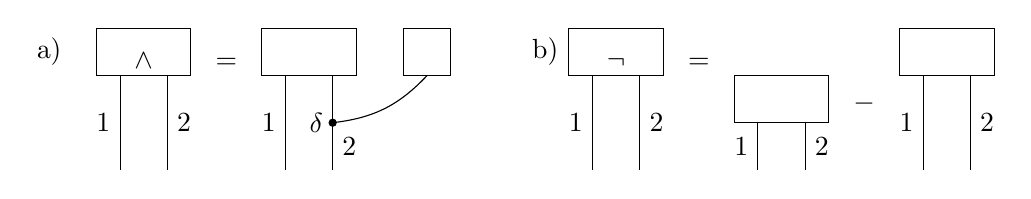
\begin{tikzpicture}[scale=0.3] 

\node at (-12,2) [above]  {a)};

	\begin{scope}[shift={(-7,0)}]
	  	\draw[]  (-3,2) rectangle (1,4);
		\node at (-1,1.9) [above] {${\exformula\land\secexformula}$};
		\draw (-2,2) -- (-2,-2) node[midway,left] {$\catvariableof{1}$};
		\draw (0,2) -- (0,-2) node[midway,right] {$\catvariableof{2}$};	
	\end{scope}
	\node at (-4.5,1.9) [above] {$=$};	
  	\draw[] (-3,2) rectangle (1,4);
	\node at (-1,1.9) [above] {${\exformula}$};
  	\draw[] (3,2) rectangle (5,4);
	\node at (4,1.9) [above] {${\secexformula}$};
	
	\node at (0,0) [left,] {$\delta$};
	\draw[]  (0,2) -- (0,0);% node[midway,left] {$\placeholderof{1}$};
	\draw[fill,] (0,0) circle (0.15cm);
	\draw[] (0,0) -- (0,-2) node[midway,right] {$\catvariableof{2}$};
	\draw[] (4,2) to[bend left=20] (0,0);
	\draw[] (-2,2) -- (-2,-2) node[midway,left] {$\catvariableof{1}$};

\begin{scope}[shift={(27,0)}]
	\node at (-18,2) [above]  {b)};
  	\begin{scope}[shift={(-14,0)}]
	  	\draw[]  (-3,2) rectangle (1,4);
		\node at (-1,1.9) [above] {${\lnot\exformula}$};
		\draw (-2,2) -- (-2,-2) node[midway,left] {$\catvariableof{1}$};
		\draw (0,2) -- (0,-2) node[midway,right] {$\catvariableof{2}$};	
	\end{scope}
	
    	\begin{scope}[shift={(-2,-2)}]
  		\draw[] (-8,2) rectangle (-4,4);
		\node at (-6,2) [above,] {$\ones$};
		\draw[] (-7,2) -- (-7,0) node[midway,left] {$\catvariableof{1}$};
		\draw[] (-5,2) -- (-5,0) node[midway,right] {$\catvariableof{2}$};
	\end{scope}
	
	\draw[] (-2,2) -- (-2,-2) node[midway,left] {$\catvariableof{1}$};
	\draw[](0,2) -- (0,-2) node[midway,right] {$\catvariableof{2}$};
	\node[] at (-4.5,0) [above] {$-$};



	\node at (-11.5,1.9) [above] {$=$};	
	
  	\draw[]  (-3,2) rectangle (1,4);
	\node at (-1,1.9) [above] {${\exformula}$};	
	
\end{scope}

\end{tikzpicture}
\end{center}
\caption{Decomposition schemes by effective calculus, using coordinatewise transforms of tensors (see \defref{def:coordinatewiseTransform}).
	a) Conjunction performed by coordinatewise multiplications, b) Negations performed by coordinatewise substraction from one.}\label{fig:ConNegDecomposition}
\end{figure}

\begin{theorem}\label{the:effectiveConjunction}
	For any formulas $\exformula,\secexformula$ we have
	\begin{align*}
		\sbcontractionof{
			\rencodingofat{\land}{\headvariableof{\exformula\land\secexformula},\catvariableof{\exformula},\catvariableof{\secexformula}},\tbasisat{\headvariableof{\exformula\land\secexformula}}
		}{\catvariableof{\exformula},\catvariableof{\secexformula}}
		= \tbasisat{\catvariableof{\exformula}} \otimes \tbasisat{\catvariableof{\secexformula}} \, .
	\end{align*}
	In particular, it holds that (see Figure~\ref{fig:ConNegDecomposition}a)
	\begin{align*}
		(\exformula\land\secexformula)[\shortcatvariables] = \sbcontractionof{\exformula,\secexformula}{\shortcatvariables} \, .
	\end{align*}
\end{theorem}
\begin{proof}
	We decompose
	\begin{align*}
		\rencodingofat{\land}{\headvariableof{\exformula\land\secexformula},\catvariableof{\exformula},\catvariableof{\secexformula}}
		= \tbasisat{\headvariableof{\exformula\land\secexformula}} \otimes \tbasisat{\catvariableof{\exformula}} \otimes \tbasisat{\catvariableof{\secexformula}}
		+ \fbasisat{\headvariableof{\exformula\land\secexformula}} \left( \onesat{\catvariableof{\exformula},\catvariableof{\secexformula}} -  \tbasisat{\catvariableof{\exformula}} \otimes \tbasisat{\catvariableof{\secexformula}} \right)
	\end{align*}
	and get the first claim as
	\begin{align*}
		\sbcontractionof{
			\rencodingofat{\land}{\headvariableof{\exformula\land\secexformula},\catvariableof{\exformula},\catvariableof{\secexformula}},\tbasisat{\headvariableof{\exformula\land\secexformula}}
		}{\catvariableof{\exformula},\catvariableof{\secexformula}}
		& = \sbcontractionof{
			\tbasisat{\headvariableof{\exformula\land\secexformula}} \otimes \tbasisat{\catvariableof{\exformula}} \otimes \tbasisat{\catvariableof{\secexformula}},\tbasisat{\headvariableof{\exformula\land\secexformula}}
		}{\catvariableof{\exformula},\catvariableof{\secexformula}} \\
		& = \tbasisat{\catvariableof{\exformula}} \otimes \tbasisat{\catvariableof{\secexformula}} \, .
	\end{align*}
	To show the second claim we use
	\begin{align*}
		(\exformula\land\secexformula)[\shortcatvariables]
		&= \sbcontractionof{
			\rencodingofat{\exformula}{\catvariableof{\exformula},\shortcatvariables},
			\rencodingofat{\secexformula}{\catvariableof{\secexformula},\shortcatvariables},
			\rencodingofat{\land}{\headvariableof{\exformula\land\secexformula},\catvariableof{\exformula},\catvariableof{\secexformula}},
			\tbasisat{\headvariableof{\exformula\land\secexformula}}
			}{\shortcatvariables} \\
		&  = \sbcontractionof{
			\rencodingofat{\exformula}{\catvariableof{\exformula},\shortcatvariables},
			\rencodingofat{\secexformula}{\catvariableof{\secexformula},\shortcatvariables},
			(\tbasisat{\catvariableof{\exformula}}\otimes \tbasisat{\catvariableof{\secexformula}})
			%\rencodingofat{\land}{\catvariableof{\exformula},\catvariableof{\secexformula},\headvariableof{\exformula\land\secexformula}}
			}{\shortcatvariables} \\
		&= \sbcontractionof{\exformula,\secexformula}{\shortcatvariables} \, .
	\end{align*}
\end{proof}

A similar decomposition holds for negations, as we show next.

\begin{theorem}
	For any formula $\exformula$ we have
	\begin{align*}
		\sbcontractionof{
			\rencodingofat{\lnot}{\headvariableof{\lnot\exformula},\catvariableof{\exformula}},\tbasisat{\headvariableof{\lnot\exformula}}
		}{\catvariableof{\exformula}}
		= \fbasisat{\catvariableof{\exformula}} =  \onesat{\catvariableof{\exformula}} - \tbasisat{\catvariableof{\exformula}} \, .
	\end{align*}
	and
	\begin{align*}
		\sbcontractionof{
			\rencodingofat{\lnot}{\catvariableof{\exformula},\headvariableof{\lnot\exformula}},\fbasisat{\headvariableof{\lnot\exformula}}
		}{\catvariableof{\exformula}}
		= \tbasisat{\catvariableof{\exformula}} \, .
	\end{align*}
	In particular, it holds that (see Figure~\ref{fig:ConNegDecomposition}b)
	\begin{align*}
		(\lnot\exformula)[\shortcatvariables] = \onesat{\shortcatvariables} - \formulaat{\shortcatvariables}  \, .
	\end{align*}
\end{theorem}
\begin{proof}
	Using that for two dimensional variables we have $\onesat{\catvariable}=\fbasisat{\catvariable}+\tbasisat{\catvariable}\, .$
\end{proof}

% Usage
These theorems provide a mean to represent logical formulas by sums of one-hot encodings.
Since any propositional formula can be represented by compositions of negations and conjunctions, they are universal.
We further notice, that the resulting decomposition is a basis+ CP format, as further discussed in \charef{cha:sparseCalculus}.
In Figure~\ref{fig:DecompositionExample} we provide an example of this decomposition.


\begin{figure}
\begin{center}
	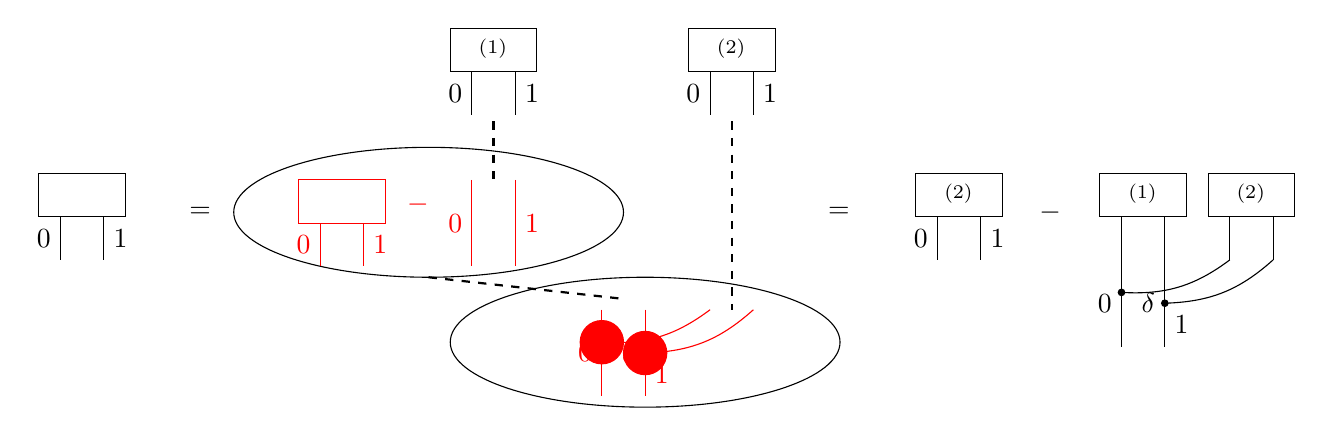
\begin{tikzpicture}[scale=0.275] % , baseline = -3.5pt



\begin{scope}[shift={(-19,-1.7)}]
		%\draw[] (-1,2.2) ellipse (4 and 2.5);
	  	\draw  (-3,2) rectangle (1,4);
		\node at (-1,1.9) [above] {${\exformula}$};
		\draw (-2,2) -- (-2,0) node[midway,left] {$\catvariableof{0}$};
		\draw (0,2) -- (0,0) node[midway,right] {$\catvariableof{1}$};	
		\node at (3.5,2.2)[right]  {$=$};
\end{scope}

\draw[] (-4,0.5) ellipse (9 and 3);
   	\begin{scope}[shift={(-2,-2)}]
  		\draw[\skeletoncolor] (-8,2) rectangle (-4,4);
		\node at (-6,2) [above,\skeletoncolor] {$\ones$};
		\draw[\skeletoncolor] (-7,2) -- (-7,0) node[midway,left] {$\catvariableof{0}$};
		\draw[\skeletoncolor] (-5,2) -- (-5,0) node[midway,right] {$\catvariableof{1}$};
	\end{scope}
	
	\draw[\skeletoncolor] (-2,2) -- (-2,-2) node[midway,left] {$\catvariableof{0}$};
	\draw[\skeletoncolor](0,2) -- (0,-2) node[midway,right] {$\catvariableof{1}$};
	\node[\skeletoncolor] at (-4.5,0) [above] {$-$};
\draw[thick,dashed] (-4,-2.5) -- (5,-3.5);
%\draw[] (6,-2.5) -- (1,-2.5);

%% Into negation core
\draw[thick,dashed] (-1,4.7) -- (-1,2);%-4,3.5);

%% Into conjunction core
\draw[thick,dashed] (10,4.7) -- (10,-4);%(6,-2.5);


\begin{scope}[shift={(10,-6)}]
	\draw[] (-4,0.5) ellipse (9 and 3);
	\begin{scope}[shift={(-4,0)}]
		\renewcommand{\skeletoncolor}{red}
	\node at (0,0) [left,\skeletoncolor] {$\delta$};
	\draw[\skeletoncolor]  (0,2) -- (0,0);% node[midway,left] {$\placeholderof{1}$};
	\draw[fill,\skeletoncolor] (0,0) circle (\dotsize);
	\draw[\skeletoncolor] (0,0) -- (0,-2) node[midway,right] {$\catvariableof{1}$};
	\draw[\skeletoncolor] (5,2) to[bend left=20] (0,0);


	\draw[fill,\skeletoncolor] (-2,0.5) circle (\dotsize);
	\draw[\skeletoncolor] (3,2) to[bend left=20] (-2,0.5);
	\draw[\skeletoncolor] (-2,2) -- (-2,-2) node[midway,left] {$\catvariableof{0}$};
	\end{scope}
\end{scope}



\begin{scope}[shift={(0,5)}]
		%\draw[] (-1,2.2) ellipse (4 and 2.5);
	  	\draw  (-3,2) rectangle (1,4);
		\node at (-1,1.9) [above] {${\secexformula^{(1)}}$};
		\draw (-2,2) -- (-2,0) node[midway,left] {$\catvariableof{0}$};
		\draw (0,2) -- (0,0) node[midway,right] {$\catvariableof{1}$};	
\end{scope}

\begin{scope}[shift={(11,5)}]
		%\draw[] (-1,2.2) ellipse (4 and 2.5);
	  	\draw  (-3,2) rectangle (1,4);
		\node at (-1,1.9) [above] {${\secexformula^{(2)}}$};
		\draw (-2,2) -- (-2,0) node[midway,left] {$\catvariableof{0}$};
		\draw (0,2) -- (0,0) node[midway,right] {$\catvariableof{1}$};	
		
\end{scope}




\node at (14,0.5)[right]  {$=$};


\begin{scope}[shift={(29,0)}]

\begin{scope}[shift={(-7.5,-1.7)}]
		%\draw[] (-1,2.2) ellipse (4 and 2.5);
	  	\draw[]  (-3,2) rectangle (1,4);
		\node at (-1,1.9) [above] {${\secexformula^{(2)}}$};
		\draw[] (-2,2) -- (-2,0) node[midway,left] {$\catvariableof{0}$};
		\draw[] (0,2) -- (0,0) node[midway,right] {$\catvariableof{1}$};	
		\node at (2.25,2.2)[right]  {$-$};		
\end{scope}


\begin{scope}[shift={(1,-3.7)}]
%	\renewcommand{\skeletoncolor}{\conjunctioncolor}
	\node at (0,0) [left] {$\delta$};
	\draw[]  (0,2) -- (0,0);% node[midway,left] {$\placeholderof{1}$};
	\draw[fill] (0,0) circle (0.15cm);
	\draw[] (0,0) -- (0,-2) node[midway,right] {$\catvariableof{1}$};
	\draw[] (5,2) to[bend left=20] (0,0);


	\draw[fill] (-2,0.5) circle (0.15cm);
	\draw[] (3,2) to[bend left=20] (-2,0.5);
	\draw[] (-2,2) -- (-2,-2) node[midway,left] {$\catvariableof{0}$};
\end{scope}


\begin{scope}[shift={(1,-1.7)}]
		%\draw[] (-1,2.2) ellipse (4 and 2.5);
	  	\draw  (-3,2) rectangle (1,4);
		\node at (-1,1.9) [above] {${\secexformula^{(1)}}$};
		\draw[] (-2,2) -- (-2,0); % node[midway,left] {$\catvariableof{0}$};
		\draw[] (0,2) -- (0,0); % node[midway,right] {$\catvariableof{1}$};	
	
\end{scope}
	
\begin{scope}[shift={(6,-1.7)}]
		%\draw[] (-1,2.2) ellipse (4 and 2.5);
	  	\draw[]  (-3,2) rectangle (1,4);
		\node at (-1,1.9) [above] {${\secexformula^{(2)}}$};
		\draw[]  (-2,2) -- (-2,0); % node[midway,left] {$\catvariableof{0}$};
		\draw[]  (0,2) -- (0,0); % node[midway,right] {$\catvariableof{1}$};	
	
\end{scope}

\end{scope}



	
	
\end{tikzpicture}
\end{center}
\caption{
	Example of a decomposition by effective calculus of a formula $\exformula(\catvariableof{1},\catvariableof{2}) = \textcolor{blue}{\lnot} \secexformula^{(1)}(\catvariableof{1},\catvariableof{2}) \textcolor{red}{\land}  \secexformula^{(2)}(\catvariableof{1},\catvariableof{2})$ into a sum of contractions.}
	\label{fig:DecompositionExample}
\end{figure}


% Calculus against the direction
\red{In an alternative perspective, effective calculus amounts to an contraction against the directionality of the relational encodings.}
For specific functions, slices of the relational encodings with respect to head variables are basis vectors.
In that case, we can perform basis calculus in the inverse direction than suggested by the directions of the tensors.
We examplify this situation in the following theorem for relational encodings of logical conjunctions and negations.




\sect{Applications in Machine Learning}

The neural paradigm of Machine Learning describes the relevance of sparse function to be effective models in the sense of learning and approximation.

% Neural Paradigm by Tensor Network Decompositions
Our model of the neural paradigm are tensor network decompositions, seen as decomposition of functions into smaller functions, which take each other as input.
Summations along input axis are avoided, when having directed and boolean tensor networks with basis calculus interpretation.

% Basis Calculus
We have already observed in Theorem~\ref{the:basisCalculus}, that the value of discrete maps can be calculated by contractions of the directed boolean relation encodings.
This has been framed as Basis Calculus.
What is more, tensor network decompositions into directed boolean tensors correspond with representation of functions as compositions of smaller functions.
We can understand each composition as marking a neuron in an architecture and thus have established a neural perspective on boolean directed tensor networks.
